\documentclass[mathserif]{beamer}
%\usefonttheme{serif}
\usepackage{xeCJK}
\usepackage{fontspec}
\usepackage{graphicx}
\usepackage{listings}
\usepackage{xcolor}
\usepackage{indentfirst}
\usepackage{tikz}
\usepackage{amssymb}
\usepackage{amsthm}
\usepackage{amsmath}
\usepackage{tabularx}
\usepackage{hyperref}
\usepackage{ulem}
\usepackage{version}
\usepackage{thmtools}
\usepackage{qtree}
\usepackage{algpseudocode}
\usepackage{mathtools}
\usepackage{multicol}
\usepackage{xcolor}

\AtBeginDocument{%
    % \DeclareSymbolFont{pureletters}{T1}{lmr}{\mddefault}{it}%
    \DeclareSymbolFont{pureletters}{OML}{cmm}{m}{it}%
    \SetSymbolFont{pureletters}{bold}{OML}{cmm}{b}{it}%   
}

\XeTeXlinebreaklocale "zh"
\XeTeXlinebreakskip = 0pt plus 1pt

\setCJKmainfont{NotoSansTC-Regular}
\setmainfont{NotoSansTC-Regular}
\usetikzlibrary{arrows,decorations.markings,decorations.pathreplacing}
\newenvironment{Hint}{\noindent\textbf{Hint.}}{}

\tikzstyle {graph node} = [circle, draw, minimum width=1cm]
\tikzset{edge/.style = {decoration={markings,mark=at position 1 with %
            {\arrow[scale=2,>=stealth]{>}}},postaction={decorate}}}

\lstset{
    basicstyle=\ttfamily\normalsize,
    numberstyle=\normalsize,
    numbers=left,
    stepnumber=1,
    numbersep=3pt,
    commentstyle=\color{black!50},
    keywordstyle=\color{white!0!blue},
    stringstyle=\color{black!50!green},
    showspaces=false,
    showstringspaces=false,
    showtabs=false,
    tabsize=4,
    captionpos=b,
    breaklines=true,
    breakatwhitespace=false,
    escapeinside={\%*}{*)},
    morekeywords={*}
}

\AtBeginSection[]{
  \begin{frame}
  \vfill
  \centering
  \begin{beamercolorbox}[sep=8pt,center,shadow=true,rounded=false]{title}
    \usebeamerfont{title}\insertsectionhead\par%
  \end{beamercolorbox}
  \vfill
  \end{frame}
}

\title{競賽程式導論}
\author{陳柏安}
\subtitle{社團報告}
\date{2023-04-07}

\usetheme{Madrid}
\usecolortheme{default}
\setbeamertemplate{itemize items}[square]
\setbeamertemplate{enumerate items}[default]
\setbeamertemplate{blocks}[default]
\lstdefinestyle{myStyle}{
    belowcaptionskip=1\baselineskip,
    breaklines=true,
    frame=none,
    numbers=none, 
    basicstyle=\footnotesize\ttfamily,
    keywordstyle=\bfseries\color{green!40!black},
    commentstyle=\itshape\color{purple!40!black},
    identifierstyle=\color{blue},
    backgroundcolor=\color{gray!10!white},
}

\begin{document}
    \frame{\titlepage}

    \begin {frame}
        \tableofcontents 
    \end {frame}

        \section{關於我}

    \begin {frame}
    \frametitle{關於我}
        \begin {itemize}
        \item 高二庚班\ 陳柏安
        \item 2022 中投區學科能力競賽\ 佳作
        \item 常用的handle: gary\_cba
        \item 被耽誤的競程選手
        \end {itemize}
    \end {frame}

        \section{競賽程式}
        
    \begin {frame}
        \frametitle{大家對競賽程式的印象是?}
        \begin {itemize}
            \item 攻破別人電腦 ?!
            \pause
            \item 比誰的程式寫的比較長 ?!
            \pause
            \item 寫一個軟體?!
            \pause 
            \item 根本不知道 !!!
            \pause
        \end {itemize}
    \end{frame}

    \begin{frame}
        \frametitle{競賽程式是什麼}
        \begin{itemize}
            \item 又稱為演算法競賽
            \pause
            \item 我們常常將競賽程式講成 競程
            \pause
            \item 主要是在比誰能在時間內解出最多、最有效率的程式
            \pause
            \item 題目內容涉及資料結構和演算法的運用
            \pause
            \item 輸入 -> 程式運算 -> 輸出
        \end{itemize}
    \end{frame}

    \begin{frame}
        \frametitle{演算法和資料結構又是什麼?}
        \begin{center}
            程式設計 = 演算法 + 資料結構
        \end{center}

        \begin{itemize}
            \item 程式語言(C++, Python, Java...)為工具
            \pause
            \item 資料結構資料儲存方式及架構
            \pause
            \item 演算法是有效率解決問題的方法
            
        \end{itemize}

    \end{frame}

    \begin{frame}
        \frametitle{太抽象? 舉個例子}
        \begin{itemize}
            \item Google 導航尋找最短的路徑
            \item 要排序一堆亂數
        \end{itemize}
        \begin{figure}[H]
            \flushright
            \centering
            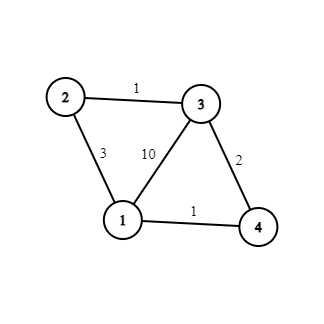
\includegraphics[width=0.5\textwidth]{graph} 
        \end{figure}
    \end{frame}

    \begin{frame}
        \frametitle{有哪些競賽?}
        \begin{itemize}
            \item 國際資訊奧林匹亞 IOI \& 台灣資訊奧林匹亞 TOI
            \item 資訊學科能力競賽\ 區賽\&全國
            \item 網際網路程式設計全國競賽 NPSC
            \item 大學程式能力先修檢測 APCS
            \item 少年圖林計畫 YTP
            \item 成功大學高中生程式設計邀請賽 NCKU
        \end{itemize}
    \end{frame}

    \begin{frame}
        \frametitle{有哪些活動可以參加?}
        \begin{enumerate}
            \item 課程
            \begin{itemize}
                \item 資訊之芽(語法班\&算法班)
                \item 普台程式設計培訓 (待定)
            \end{itemize}
            \item 營隊
            \begin{itemize}
                \item APCS camp
                \item IOI camp
                \item ION camp
            \end{itemize}
        \end{enumerate}
    \end{frame}

        \section{升學的新選擇}

    \begin{frame}
        \frametitle{升學不再只是學霸的天下}
        \begin{enumerate}
            \item 特殊選材
            \begin {itemize}
                \item 不用考學測
                \pause
                \item 要有出色的競賽成績,或是你很特殊
                \pause
                \item 在程式上要付出很多心力
                \pause
                \item 賭很大
            \end {itemize}
            \pause
            \item 學測-APCS組
            \begin{itemize}
                \item 還是要準備學測,標準相對的比較低
                \pause
                \item 可以說是第二次的特選
                \pause
                \item APCS 觀念4 實作 4 (以上)
            \end{itemize}
        \end{enumerate}
    \end{frame}

    \begin{frame}
        \begin{figure}[H]
            \centering
            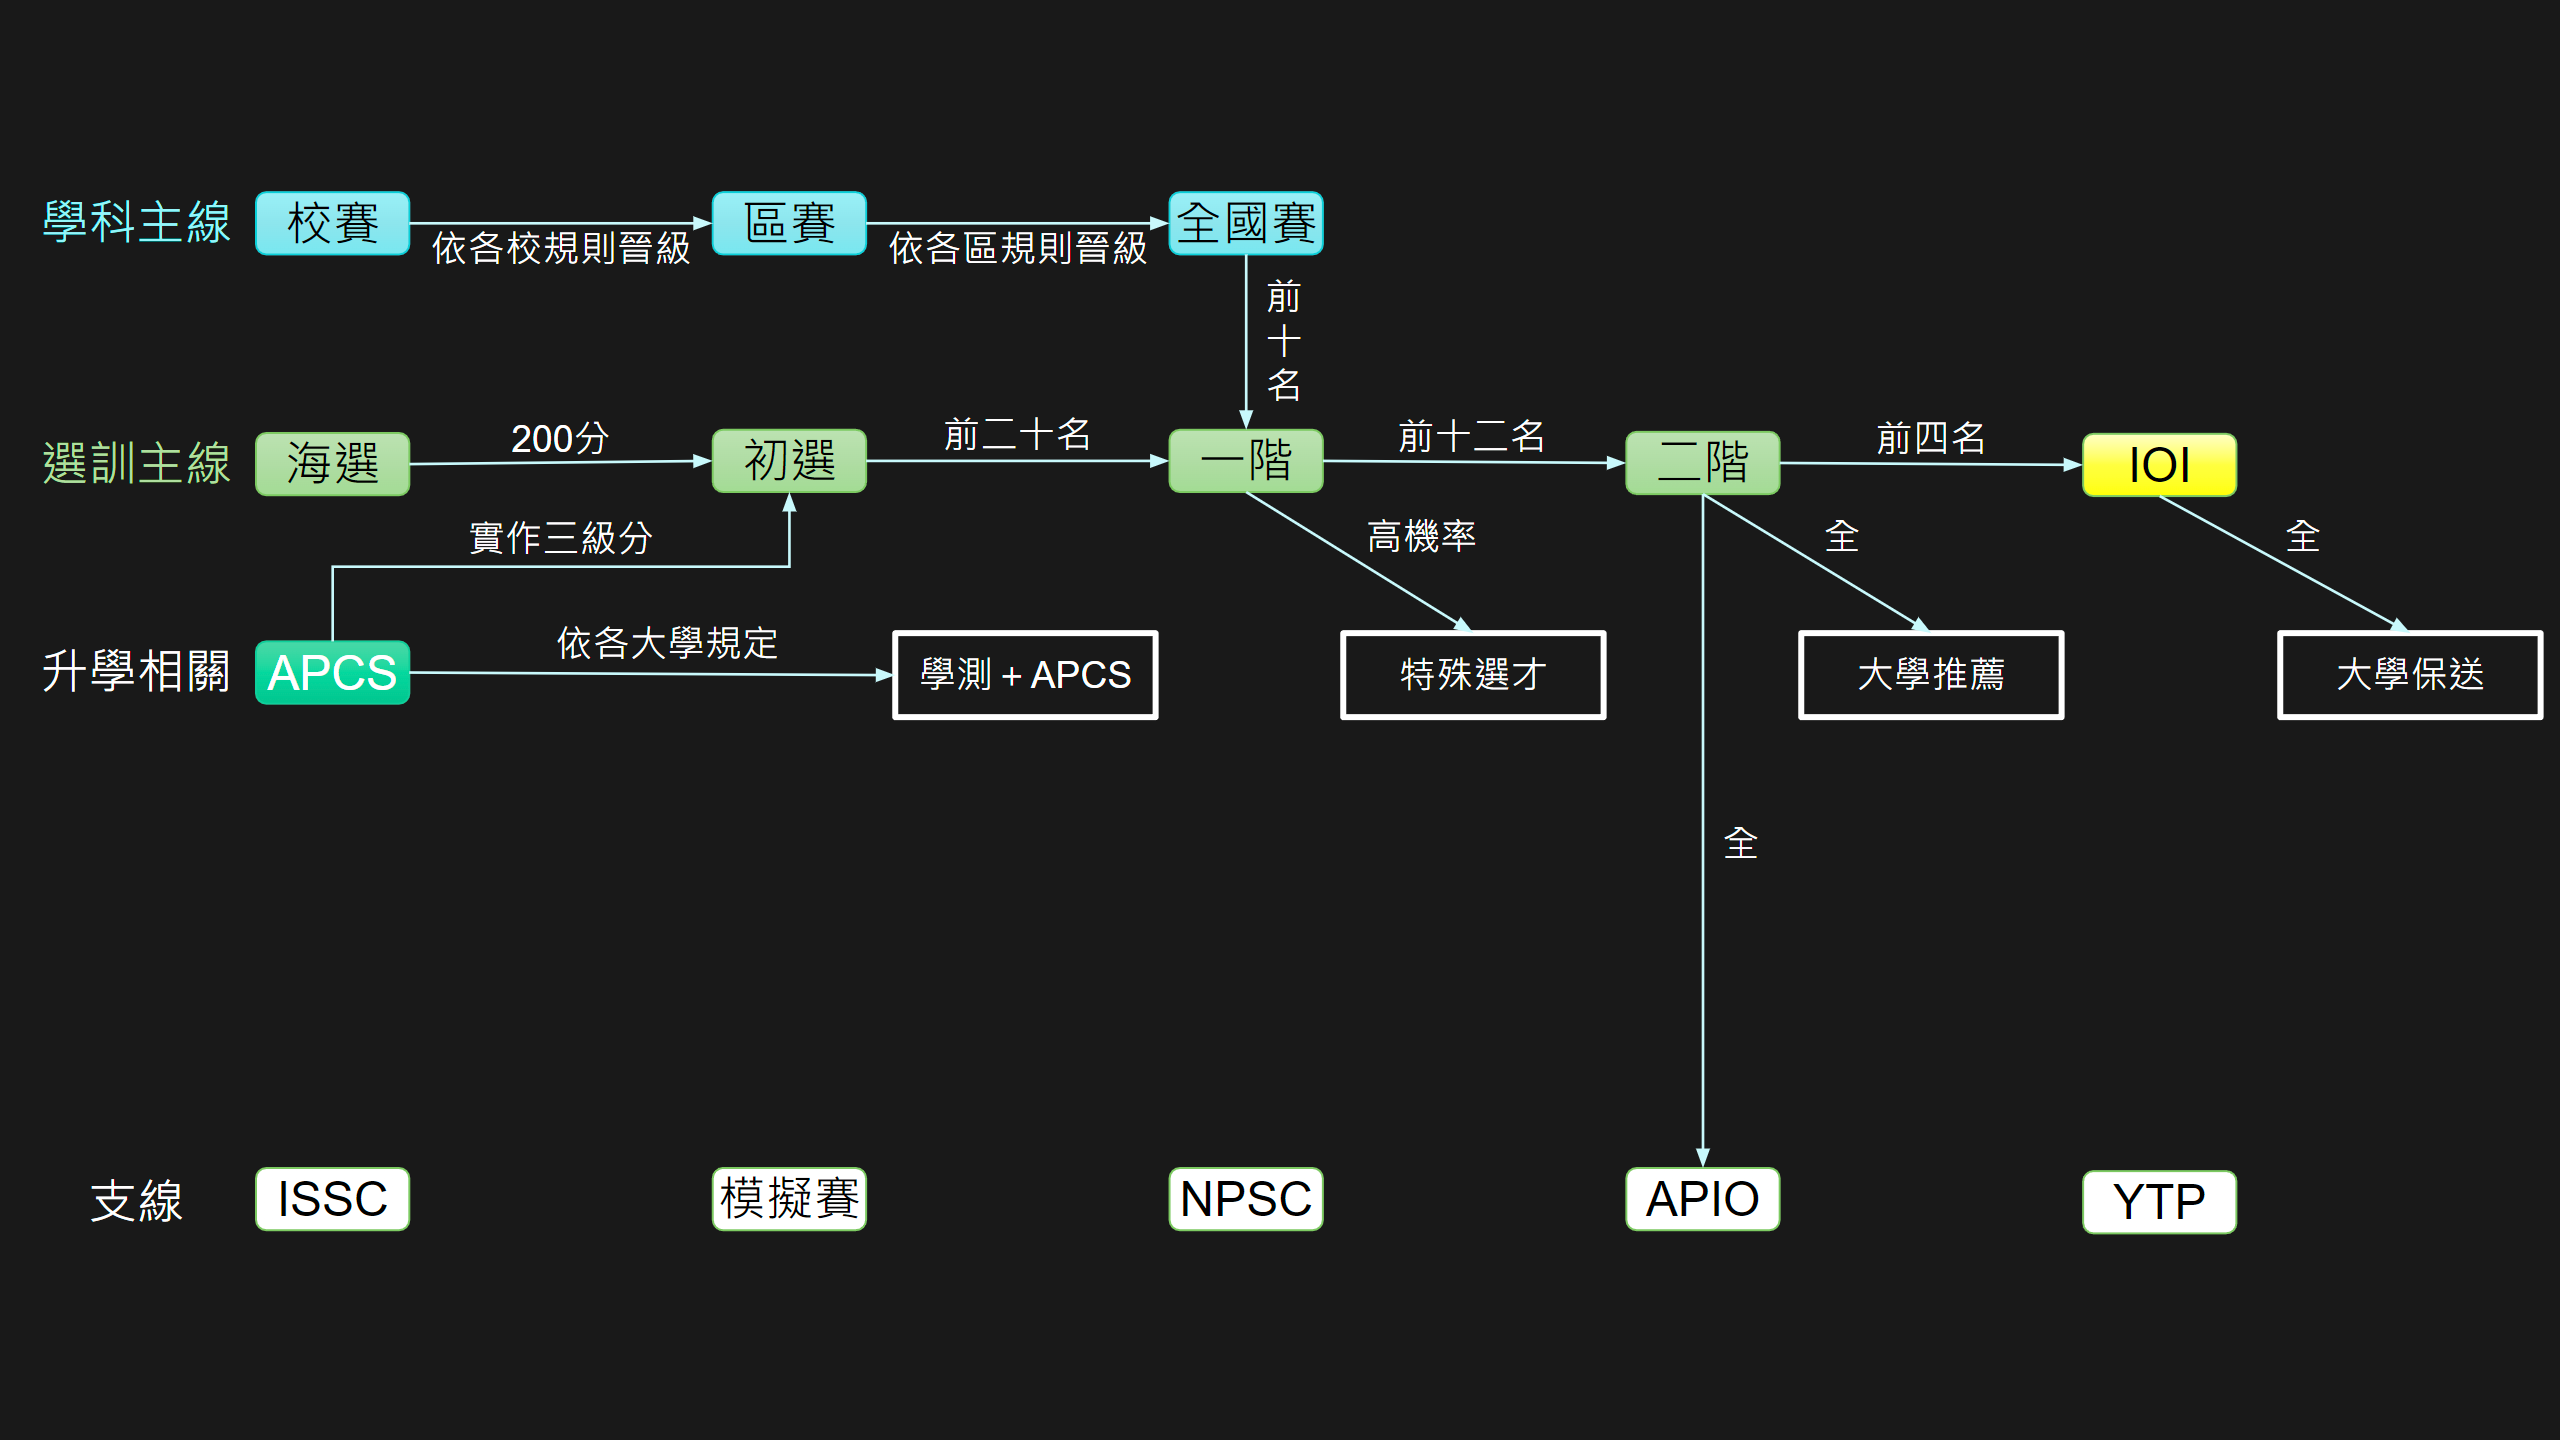
\includegraphics[width=1\textwidth]{contest} 
            \caption{競賽路線}
        \end{figure}
    \end{frame}

        \section{未來的規劃}

    \begin{frame}
        \frametitle{普台程式設計培訓計畫}
        Maker \& 競賽解題社
        \begin{itemize}
            \item 演算法課程 (須具備基礎程式能力,最好能會C++)
            \pause
            \item 有人數限制
            \pause
            \item 期中和期末測驗
            \pause
            \item 希望能夠將各位訓練成競程好手
        \end{itemize}
    \end{frame}

    \begin{frame}
        \frametitle{普台程式設計培訓計畫}
        Discord PTITC 普台資訊社群
        \begin{itemize}
            \item 互相交流、學習的地方
            \pause
            \item 邀請畢業學長姊加入(資工、電機、通訊、資管...)
            \pause
            \item 對資訊有興趣的皆可加入
        \end{itemize}
    \end{frame}

        \section{總結}
    
    \begin{frame}
        \frametitle{總結}
        \begin{itemize}
            \item 競程是一個很讚的東西
            \pause
            \item 可以訓練自己的邏輯能力、程式能力
            \pause
            \item 還能讓你多一個上大學的機會
            \pause
            \item 心動不如行動,一起加入競程的行列,一起成為普台之光(讓那些上級跌破眼鏡),一起打程式or被程式打吧!
        \end{itemize}
    \end{frame}

    \begin{frame}
        \begin{center}
            謝謝大家!
        \end{center}
    \end{frame}

\end{document}